% !TEX root = ../main.tex
%--- Slide 8: simulazione di riferimento (circa 50 s) ------------------------------------
\begin{frame}{Simulazione di riferimento}
  \begin{columns}[c]
    \column{0.55\textwidth}
    \begin{itemize}
      \item Stessi TOA, incertezze e frequenze di DR2low
      \item Residui sostituiti da una realizzazione dei soli tre processi del modello
      \item \simul{Simulazione}: parametri iniettati recuperati,\\
            un solo picco, niente L
      \item La copertura in frequenza di DR2low basta a distinguere DM e scattering
    \end{itemize}
    \column{0.42\textwidth}
    \centering
    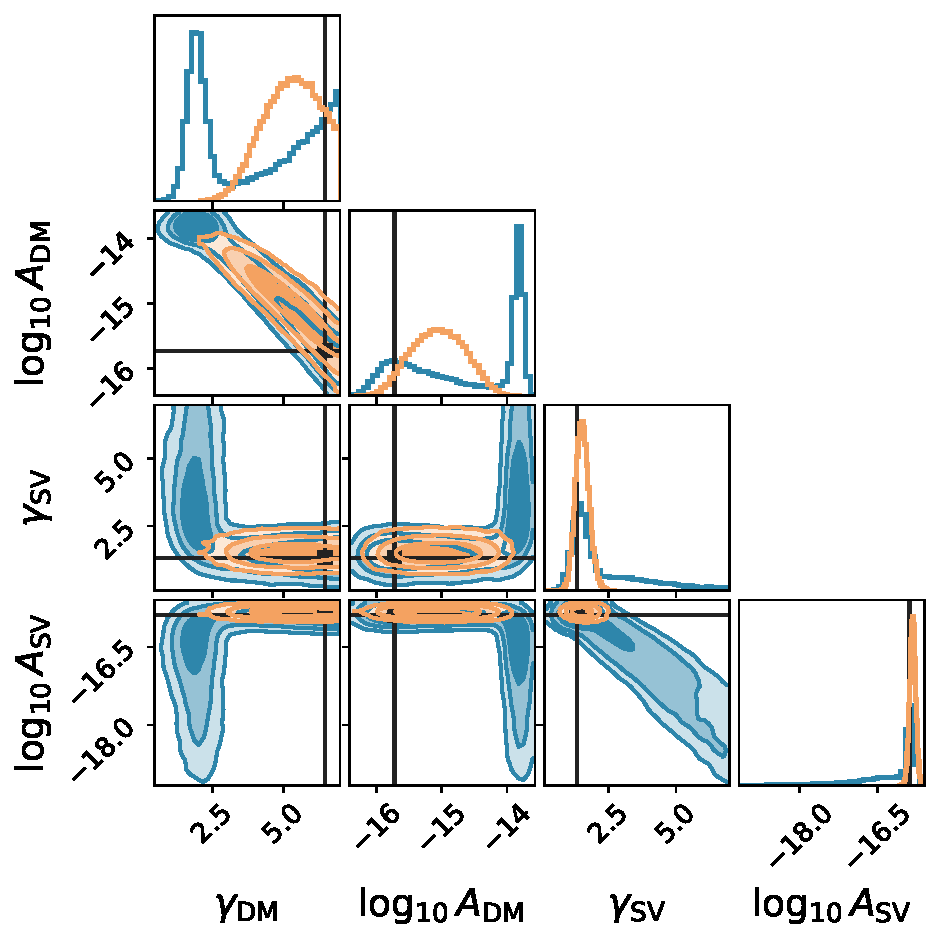
\includegraphics[height=0.72\textheight]{Figure/P08_reali_vs_sim_DM_SV.pdf}\par
    {\footnotesize \reali{dati reali} \quad \simul{simulazione}\\ linee nere: valori iniettati}
  \end{columns}
\end{frame}
